% Name: Log-log plot
% Description: Operation counts of three algorithms against input size, where power laws become straight lines.
% Tags: log-log, complexity, power law, logarithmic axes

\usepackage{pgfplots}
\pgfplotsset{compat=1.18}

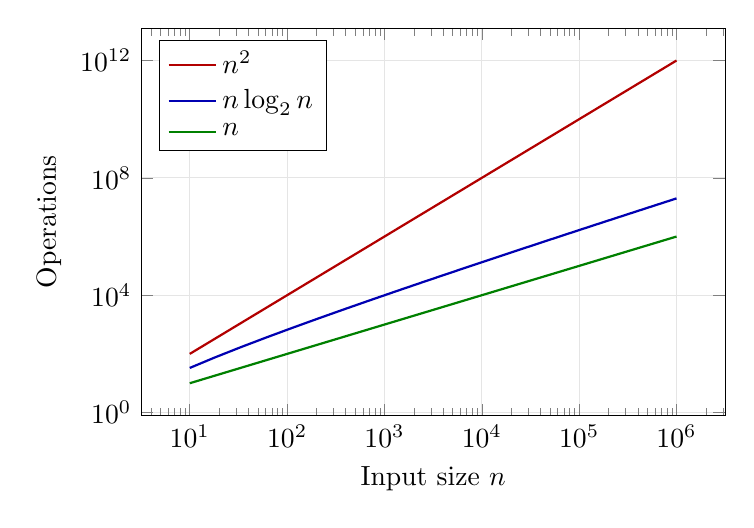
\begin{tikzpicture}
  \begin{loglogaxis}[
    width=9cm, height=6.5cm, domain=10:1e6, samples=20,
    xlabel={Input size $n$}, ylabel={Operations},
    legend pos=north west, legend cell align=left,
    grid=major, grid style={gray!20},
  ]
    \addplot[red!70!black, thick] {x^2};
    \addplot[blue!70!black, thick] {x*ln(x)/ln(2)};
    \addplot[green!50!black, thick] {x};
    \legend{$n^2$, $n \log_2 n$, $n$}
  \end{loglogaxis}
\end{tikzpicture}
